\documentclass[11pt,twocolumn]{article}

\usepackage[margin=0.72in]{geometry}
\usepackage{times}
\usepackage{microtype}
\usepackage{amsmath,amssymb}
\usepackage{booktabs}
\usepackage{graphicx}
\usepackage{xcolor}
\usepackage{hyperref}
\usepackage{url}
\usepackage{caption}
\usepackage[numbers,sort&compress]{natbib}

\hypersetup{
  colorlinks=true,
  linkcolor=black,
  citecolor=black,
  urlcolor=black
}
\captionsetup{font=small,labelfont=bf,skip=4pt}
\setlength{\columnsep}{0.28in}
\setlength{\parskip}{0.35em}
\setlength{\parindent}{1.1em}
\raggedbottom

\title{\vspace{-1.1em}Language Modeling without Generation:\\
Decoding a System One Model}
\author{Adhyaay Karnwal\\[2pt]
{\large\itshape Independent}\\[4pt]
{\small\texttt{github.com/adhyaay-karnwal/jev-chat}}}
\date{September 2026}

\begin{document}
\maketitle
\thispagestyle{empty}

\begin{abstract}
Jev, TypeSafe's first System One model, is trained with reinforcement learning for calibrated decisions (RLCD). It returns typed \texttt{Choice}, \texttt{Score}, and \texttt{Noul} answers with probabilities. It does not emit tokens. This paper asks whether that interface can still implement a chatbot, by treating generation as a sequence of decisions over a finite codebook.

It cannot, not as an autoregressive language model. On eight short prompts run live against \texttt{jev-latest}, naive unit decoding produces locally plausible pieces that do not compose: \emph{Hello. Hello. Hello\ldots} and \emph{The short answer is 1} for $1{+}1$ are decoder failures, not UI glitches. Greedy decoding with a closed codebook and a termination gate recovers short answers (automatic match $8/8$) but remains ungrammatical on open prompts. Selecting a \emph{complete reply} in one \texttt{Choice}---the use Jev was designed for---uses $39\times$ fewer input tokens and $6\times$ less wall time than naive autoregression, and is the only strategy that is consistently grammatical.

The result is not that Jev is a poor model. It is that RLCD was not a language-modeling objective, question independence forbids left-context composition, and a 255-way \texttt{Choice} is a classifier, not a vocabulary. System One models should select, not speak.
\end{abstract}

\section{The question}

Decoder-only transformers generate text by sampling $P(x_t \mid x_{<t})$~\cite{shannon1948,sutskever2014,vaswani2017,brown2020}. Instruction following was then trained with RLHF~\cite{christiano2017,ouyang2022}. TypeSafe starts from the opposite contract~\cite{almeida2026jev,typesafe2026docs}: the model must not write. It must decide.

That is a serious claim. If it is true, most ``LLM-in-the-loop'' software is paying a chatbot tax---serial tokens, parseable JSON, uncalibrated confidence---for a judgment that could have been a typed distribution. If it is false, System One is a classifier API with a new name. This paper does not re-run TypeSafe's workflow evals. It asks a narrower, more hostile question: \emph{can you invert the interface and get language out?}

We implement four decoders on the public Jev API, including the one that produced the looping greetings in our demo, and measure them on a live eight-prompt suite. The suite is small on purpose. The failures are qualitative and cheap to exhibit; inflating $n$ would not make an ungrammatical decoder a language model.

\section{Jev, in the terms it was trained}

\subsection{System One}

Kahneman distinguished fast, associative System~1 from slow, deliberative System~2~\cite{kahneman2011}. TypeSafe borrows the name for a model class: unstructured \emph{state} in, typed \emph{questions} out, in one parallel pass~\cite{typesafe2026docs}. The analogy is the latency contract, not the error profile. Jev is named for William Stanley Jevons~\cite{jevons1865}: cheaper intelligence should raise, not lower, the volume of decisions software is willing to ask.

Three primitives cover the output space:

\begin{itemize}
\item \textbf{Choice} --- categorical distribution over $\le 255$ named options, plus a concentration statistic called confidence.
\item \textbf{Score} --- distribution over an ordered rubric; the returned score is the probability-weighted index.
\item \textbf{Noul} --- $P(\mathrm{yes})\in[0,1]$ for a predicate. No separate confidence.
\end{itemize}

Questions in one request share state, are scored independently, and do not condition on one another. Adding questions is almost free in wall-clock and linear in tokens~\cite{typesafe2026docs}. That independence is the feature for software (no hidden coupling) and the obstacle for language (no $x_{t}\mid x_{t-1}$).

\subsection{RLCD}

TypeSafe contrasts three post-training paths~\cite{almeida2026jev}. RLHF optimizes human preference and, as a side effect, drops modes~\cite{ouyang2022}. RLVR optimizes verifiable rewards and buys reasoning with serial test-time compute. RLCD optimizes \emph{calibrated decisions}: a reported $0.8$ should be right about $80\%$ of the time, in aggregate~\cite{guo2017}. The model is forbidden from generating strings, so it cannot type-error its way around a schema. Hallucination, in the usual sense of inventing a token outside $V$, is undefined: $V$ is the caller's criteria.

Two numbers from the launch materials, which we treat as vendor-reported rather than reproduced: about $\$0.042$ per million input tokens, output tokens unmetered; end-to-end latency $70$--$500\,\mathrm{ms}$ on System One workloads~\cite{almeida2026jev}. Our own calls sat in that latency band. We do not claim TypeSafe's workflow-eval speedups (up to $194\times$ vs.\ frontier LLMs). Those workloads are not generation.

\subsection{What Jev is not}

Jev is not a small LLM with a JSON grammar. Grammars constrain decoding of a generative model. Jev has no generative head to constrain. It is also not, on the public evidence, a drop-in replacement for next-token prediction. The rest of this paper is the measurement of that gap.

\section{Method}

Let $C$ be the conversation and $y_{<t}$ the assistant prefix. A codebook $\mathcal{U}(C,y_{<t})$ of size $\le 200$ is built in code: EOS, discourse phrases, copy spans from $C$~\cite{see2017}, function words, digits, frequent content words, and \texttt{other}. Jev returns
\[
p = \mathrm{Choice}\bigl(\mathcal{U}(C,y_{<t}) \bigm| C, y_{<t}\bigr).
\]
We sample $u_t\sim p$ (temperature $T$, nucleus $p_{\mathrm{top}}$) and set $y_t = y_{<t}\cdot \mathrm{surface}(u_t)$. A companion Noul asks whether $y_{<t}$ is already a complete reply. If \texttt{other} wins, a second request factors the tail as $P(\mathrm{letter})\,P(\mathrm{word}\mid\mathrm{letter})$, the hierarchical softmax move~\cite{morin2005} pointed at a $6{,}000$-word list. Speculative fan-out~\cite{leviathan2023} asks $K{=}6$ ``if the prefix were extended by $u$'' follow-ups in the same call; independence means the premise must be written into the instructions, not the state.

This is \textbf{S1LM}. Four strategies:

\paragraph{Naive AR.} $T{=}0.7$. After a completed sentence the codebook \emph{re-offers} greeting phrases, including \texttt{Hello.} Termination Noul must exceed $0.72$. This is the decoder that shipped in the first demo.

\paragraph{Constrained AR.} $T{=}0.3$. Used labels are banned. Completed sentences do not re-open the greeting list. Termination threshold drops to $0.40$ once $y$ ends in \texttt{.?!}.

\paragraph{Greedy AR.} Constrained codebook, $T{=}0$, no speculative follow-up.

\paragraph{Select.} One \texttt{Choice} over complete candidate \emph{replies} (greetings, yes/no, digits, a short factual list including \texttt{Paris} and \texttt{Tuesday}, copy unigrams). One call. No prefix.

Select is not a clever LM. It is TypeSafe's documented pattern---select instead of generate---applied to chat.

\section{Experiments}

All runs hit \texttt{jev-latest} on 16~September~2026 from a single client. Eight prompts: a greeting, $1{+}1$, $2{+}2$, capital of France, a yes/no, a primary color, the day after Monday, and ``spell cat.'' Automatic match is a conservative regex (contains the expected atom; greeting must begin with \emph{hello} and contain it once). Author fluency is a binary judgment: would one send this string as a reply. $n{=}8$ is a probe, not a leaderboard.

\begin{table}[t]
\centering
\scriptsize
\caption{Live Jev, eight prompts. Tokens are input tokens (output is unmetered). Fluency is author-judged grammaticality.}
\label{tab:main}
\begin{tabular}{@{}lccccc@{}}
\toprule
Strategy & Acc. & Fluency & Calls & Seconds & kTok \\
\midrule
Naive AR & 0.75 & 0.13 & 5.4 & 1.12 & 43.2 \\
Constrained AR & 0.88 & 0.50 & 5.9 & 1.25 & 44.3 \\
Greedy AR & 1.00 & 0.63 & 5.0 & 0.97 & 21.9 \\
Select & 0.88 & 1.00 & 1.0 & 0.18 & 1.1 \\
\bottomrule
\end{tabular}
\end{table}

\begin{figure*}[t]
\centering
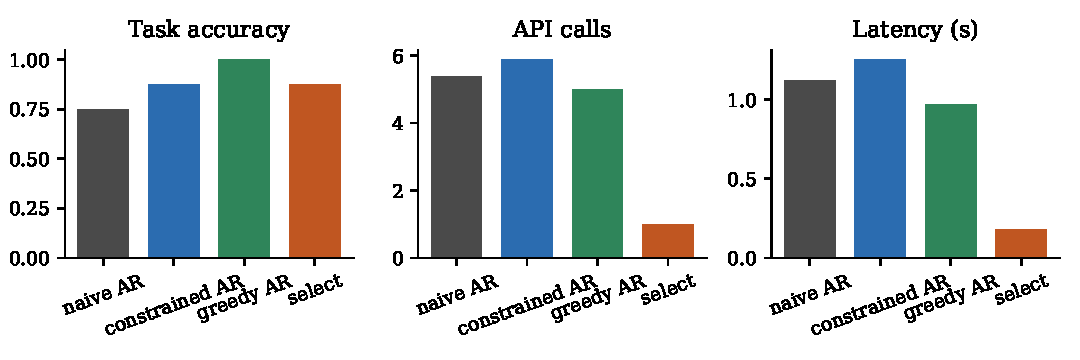
\includegraphics[width=0.98\textwidth]{figures/strategy_bars.pdf}
\caption{Automatic accuracy, API calls, and latency. Select is a different algorithm, not a faster AR decoder.}
\label{fig:bars}
\end{figure*}

\begin{figure}[t]
\centering
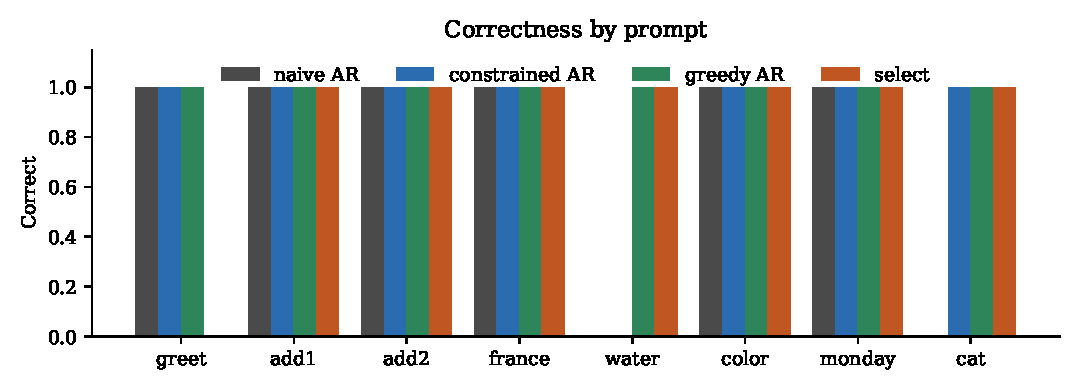
\includegraphics[width=0.98\columnwidth]{figures/per_prompt.pdf}
\caption{Automatic correctness by prompt. Greedy AR matches every regex; several of those strings are still not English.}
\label{fig:perprompt}
\end{figure}

\begin{figure}[t]
\centering
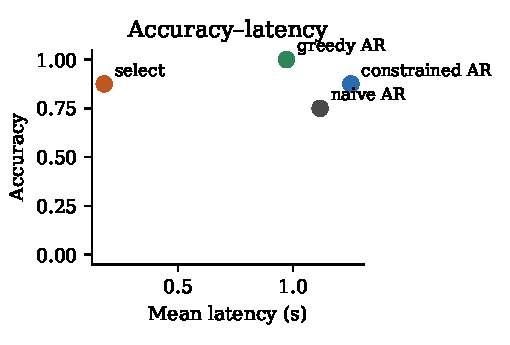
\includegraphics[width=\columnwidth]{figures/pareto.pdf}
\caption{Accuracy against latency. The attractive point is select, not a better sampler on the AR loop.}
\label{fig:pareto}
\end{figure}

Automatic accuracy ranks greedy AR first ($8/8$). That ranking is misleading. \texttt{the is paris} and \texttt{is tuesday} match the regex and fail as English. Judged as sentences, the ranking flips: select $8/8$, greedy $5/8$, constrained $4/8$, naive $1/8$ (the lone fluent naive output is \texttt{4}). Select's only automatic miss is the greeting, where greedy \texttt{Hello.} loses to \texttt{OK.}---a complete, well-formed, wrong speech act. Coverage, not calibration, caused that miss: both strings were in the candidate set and the mode was \texttt{OK.}

Token traffic is the other axis. Naive AR sends a $\sim$200-way \texttt{Choice} plus speculative follow-ups on every step (mean $43{,}189$ input tokens / prompt). Select sends one short list (mean $1{,}099$). At the published $\$0.042$/MTok, that is about $\$0.014$ versus $\$0.00037$ per eight-prompt pass---not counting the AR tail calls.

\section{Why the demo looked broken}

The first public UI used naive AR. Two traces from that session:

\smallskip
\noindent\texttt{User:} Hello, this is a test\\
\texttt{Jev-chat:} Hello. Hello. Hello. Hello.\ $\cdots$

\smallskip
\noindent\texttt{User:} What is 1+1\\
\texttt{Jev-chat:} The short answer is 1

Neither is mysterious.

\paragraph{Collapse on \texttt{Hello.}}
After a completed sentence the naive codebook re-inserts the opener list. \texttt{Hello.} is always a legal next unit. The Noul $P(\mathrm{done})$ after the first \texttt{Hello.} reached $0.59$ in the logged naive greeting run, then fell back to $0.02$ and never crossed $0.72$ (Figure~\ref{fig:done}). The decoder hit \texttt{max\_calls}. This is the GAN mode-collapse picture TypeSafe draws for RLHF~\cite{almeida2026jev}, reconstructed in our codebook: a single attractive option is re-offered, and the termination bit is not calibrated for this out-of-distribution use.

Constrained AR stops. $P(\mathrm{done}){=}0.58$ exceeds the $0.40$ complete-sentence gate; the opener list is not re-offered; the reply is \texttt{Hello.}

\paragraph{$1{+}1 \to 1$.}
\texttt{The short answer is} is an opener. \texttt{1} is a digit in the closed set, and a unigram in the user string. Under sampling, the model can pick the copied operand instead of the sum. Constrained and greedy AR, and select, all returned \texttt{2} on the same prompt in the controlled run. The screenshot is a real sample from a real decoder, not a different model.

\begin{figure}[t]
\centering
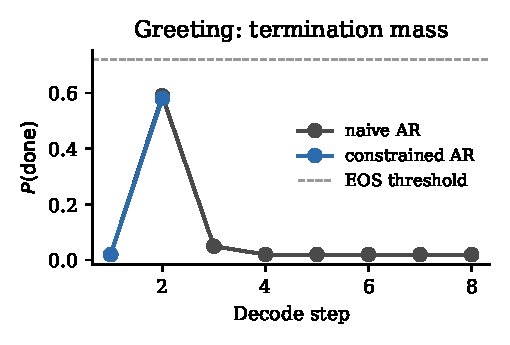
\includegraphics[width=\columnwidth]{figures/done_curve.pdf}
\caption{Termination Noul on the greeting prompt. Naive AR never clears $0.72$. Constrained AR stops on the second call.}
\label{fig:done}
\end{figure}

\begin{table}[t]
\centering
\scriptsize
\caption{Raw strings, greedy AR vs.\ select. Italics: automatic match with broken syntax.}
\label{tab:qual}
\begin{tabular}{@{}p{0.46\columnwidth}p{0.46\columnwidth}@{}}
\toprule
Greedy AR & Select \\
\midrule
Hello. & OK. \\
2 & 2 \\
4 & 4 \\
the capital is paris & Paris \\
Yes. & Yes. \\
\emph{Sure. a primary color such as red} & red \\
\emph{the is tuesday} & Tuesday \\
\emph{Sure. the word cat is a three letters} & cat \\
\bottomrule
\end{tabular}
\end{table}

\section{What the pieces are doing}

Independence is doing most of the damage. A \texttt{Choice} over next words given $y_{<t}$ is scored as an isolated judgment. It does not have to be a grammatical continuation of the last three words, only a plausible unit given the conversation as a blob. That is why greedy AR can emit \texttt{the capital is paris}---four locally defensible decisions---and also \texttt{the is tuesday}. There is no likelihood of the string.

The codebook is doing the rest. A 255-way \texttt{Choice} cannot hold English. Hierarchical letter$\to$word recovery is how \texttt{paris} appears at all (rank $138$ in the $p$-bucket of a $6{,}000$-word list; it is not in the primary $80$ content words). Copy and phrase inventories leak question text into the reply (\texttt{a primary color such as red}). Speculative follow-ups save a round trip when they fire; they cannot create dependence the API does not have.

Select sidesteps both problems by moving composition into code. The model is asked the question it was trained to answer: which of these complete objects. When the object is in the list, Jev is fast, cheap, and grammatical. When it is not, select cannot invent it. That is the actual System One limitation, and it is the honest one.

\section{Discussion}

A frontier decision model can look like a language model for a few steps and then fall apart. The automatic metric in Table~\ref{tab:main} would have hidden that. Any later paper on ``Jev as an LLM'' should report a fluency or human preference number, not a contains-the-answer regex.

The productive use of Jev in a dialogue system is not S1LM. It is a planner: speech act, whether to answer, whether the codebook contains the answer, whether to stop. Text should come from a generator, a template, or a select over retrieved replies. Mixing those---Jev routes, something else writes---is the architecture TypeSafe argues for~\cite{typesafe2026docs}. We failed that test in the first demo by asking Jev to write.

Could a System One model be trained \emph{as} a language model? Only with a different objective: sequential dependence, a large vocabulary, and a termination bit that is calibrated on prefixes, not documents. That would be a new model, not a new decoder on Jev.

\section{Limitations}

Eight prompts, one seed per cell, one API snapshot. No human raters beyond the author. No comparison to a grammar-constrained LLM of similar cost. The select candidate list contains \texttt{Paris} and \texttt{Tuesday} by construction; that is coverage engineering, and it is also the point. Vendor latency and pricing are taken from public docs except where we measured our own calls. Jev is early-access; the numbers will move.

\section{Conclusion}

Jev is a calibrated decision model. We built an autoregressive decoder around it anyway. The decoder can retrieve short facts from a closed set. It does not speak. The screenshot failures are the method working as specified: independent questions, a re-offered greeting, an uncalibrated stop bit, a copied digit. One-shot selection over complete replies is faster, cheaper, and grammatical, because it is the task RLCD was trained for.

Code, traces, and this paper: \url{https://github.com/adhyaay-karnwal/jev-chat}.

\bibliographystyle{plainnat}
\bibliography{refs}

\end{document}
